% !TeX root = ../../../proposal.tex
% Chapter 3: Methodology
\chapter{วิธีการดำเนินงาน}
\thaijustify{
  ในบทที่ 3 จะกล่าวถึงภาพรวมการออกแบบสถาปัตยกรรมระบบและแผนภาพแสดงกรณีการใช้งาน (Use case diagram) ของโครงงาน
}
\begin{samepage}
  \section{Preliminary Use Case Diagram}
  \thaijustify{
    แผนภาพกรณีการใช้งาน (Use case diagram) แสดงความสัมพันธ์ระหว่างผู้ใช้งานแต่ละบทบาทกับฟังก์ชันของแพลตฟอร์ม โดยแบ่งออกเป็น 4 ส่วน ได้แก่ ส่วน Authentication, ส่วนสร้าง two-alternative UI, ส่วนทดสอบการใช้งานและรับความเห็น, และส่วนสร้างรายงาน
  }
  \subsection{Authentication}
  \begin{figure}[H]
    \centering
    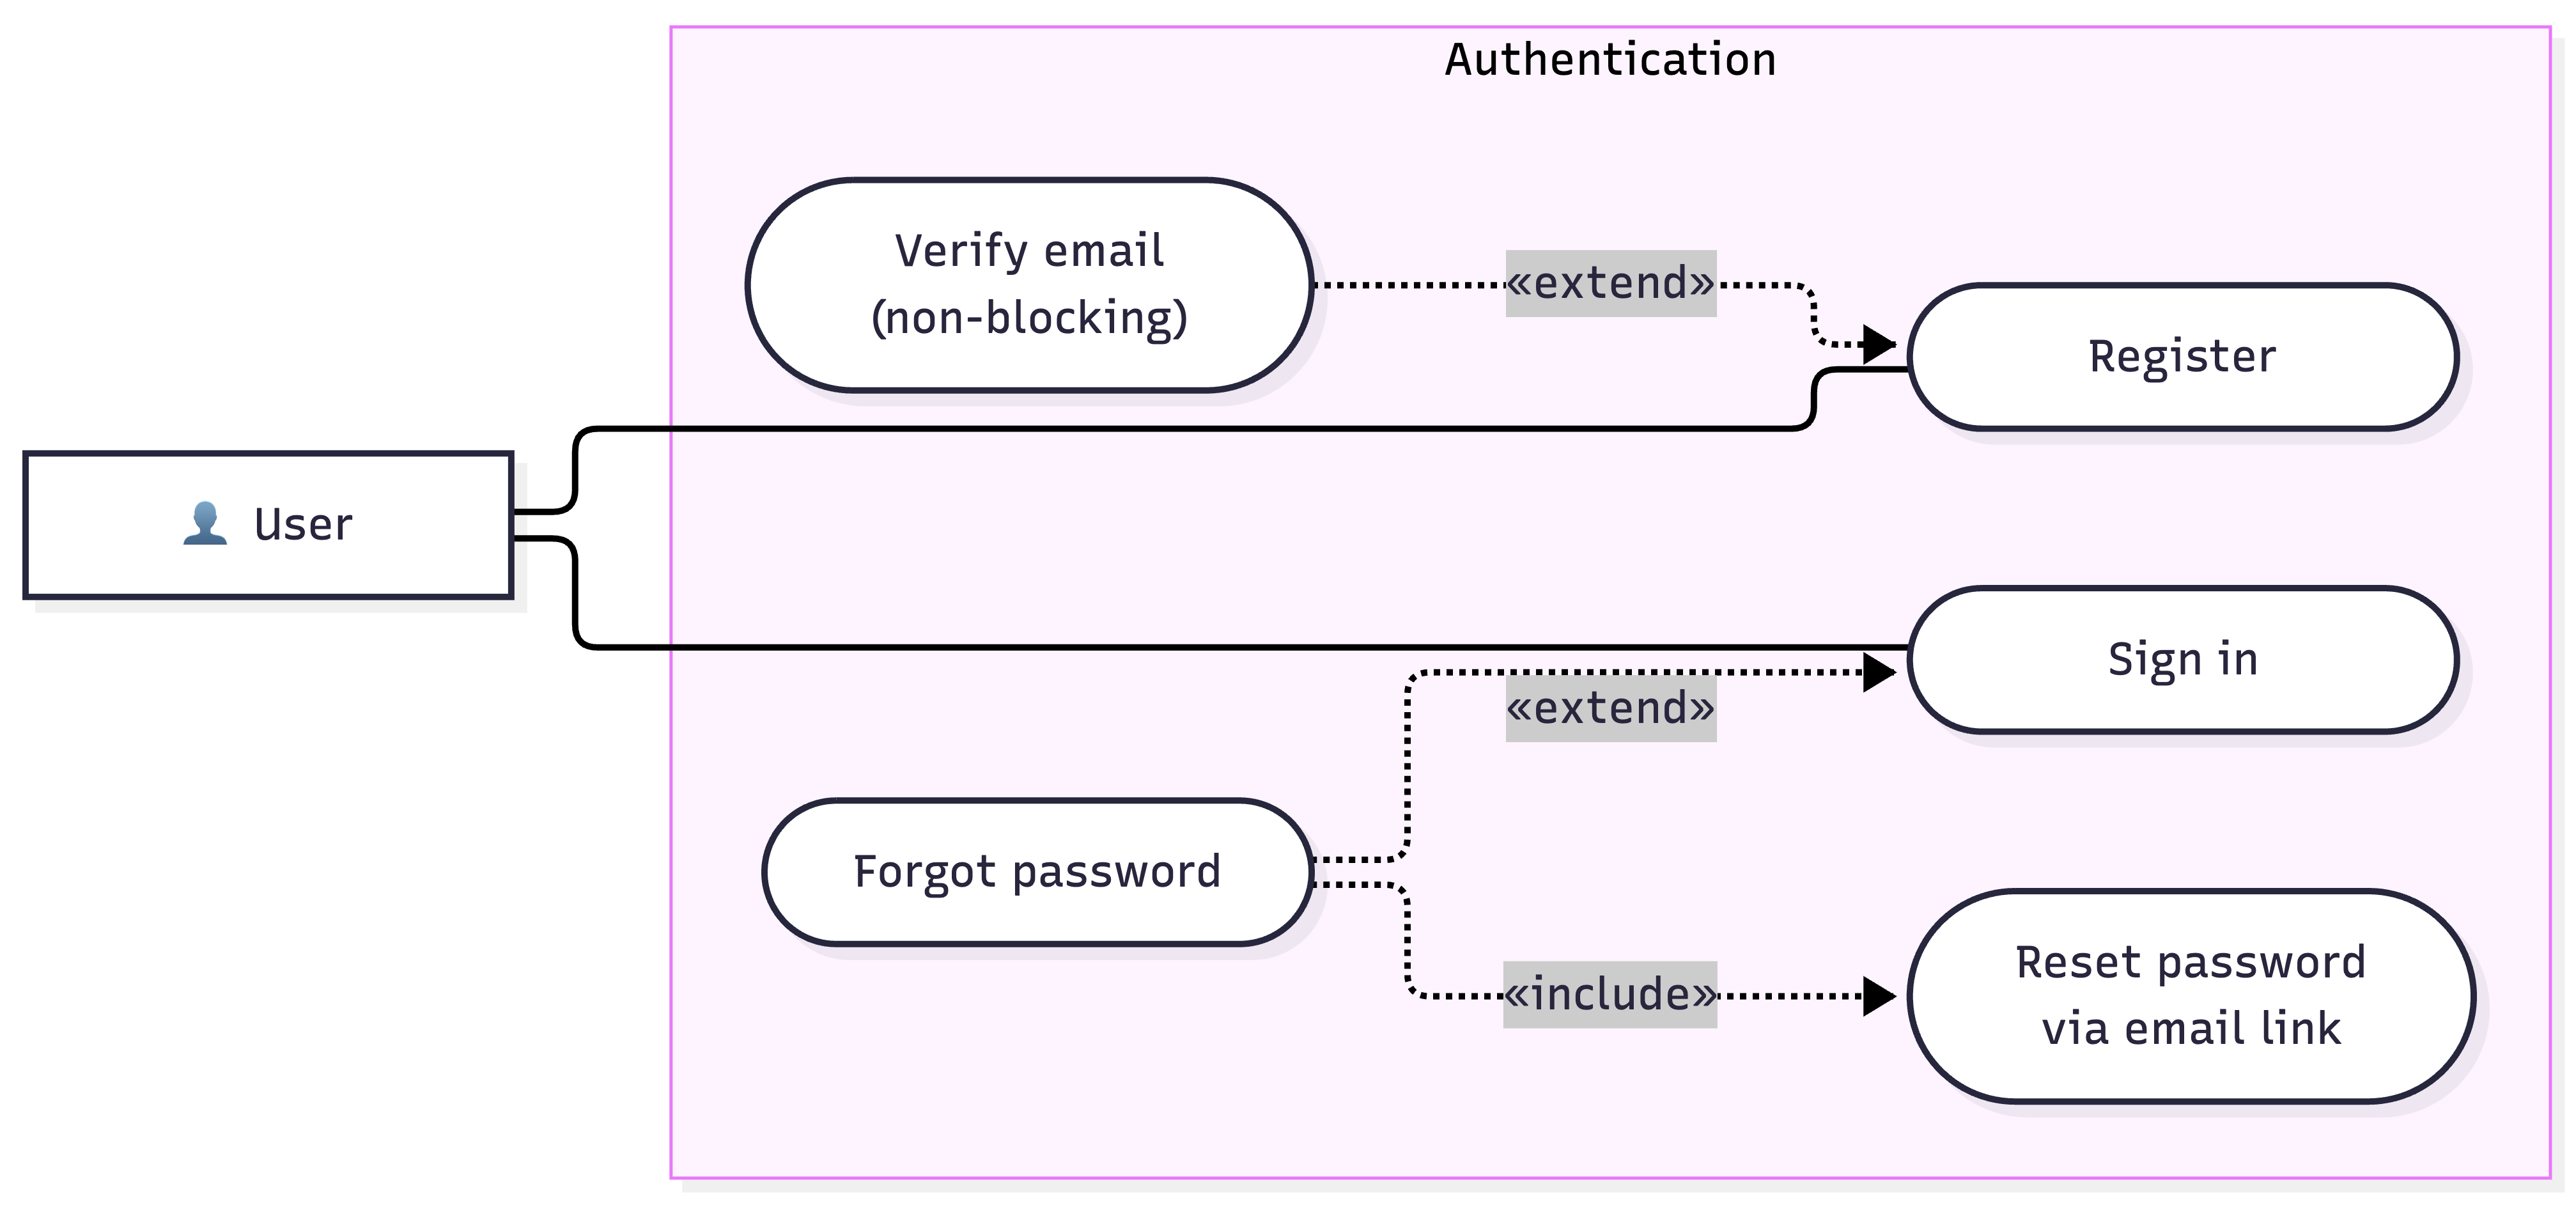
\includegraphics[
      width=0.6\textheight,
      height=\linewidth,
      keepaspectratio,
      origin=c
    ]{figures/ch3-methodology/UC-1.png}
    \caption{Use case diagram for authentication}
    \label{fig:UC-1}
    \thaijustify{ภาพแสดง Use Case ของระบบ Authentication โดยผู้ใช้สามารถสมัครสมาชิก เข้าสู่ระบบ และกู้คืนรหัสผ่านได้ โดยการยืนยันอีเมลเป็นขั้นตอนเสริมหลังการสมัคร และการรีเซ็ตรหัสผ่านดำเนินการผ่านลิงก์ที่ส่งทางอีเมล}
  \end{figure}
  \subsection{Designer: Project setup \& UI Generation}
  \begin{figure}[H]
    \centering
    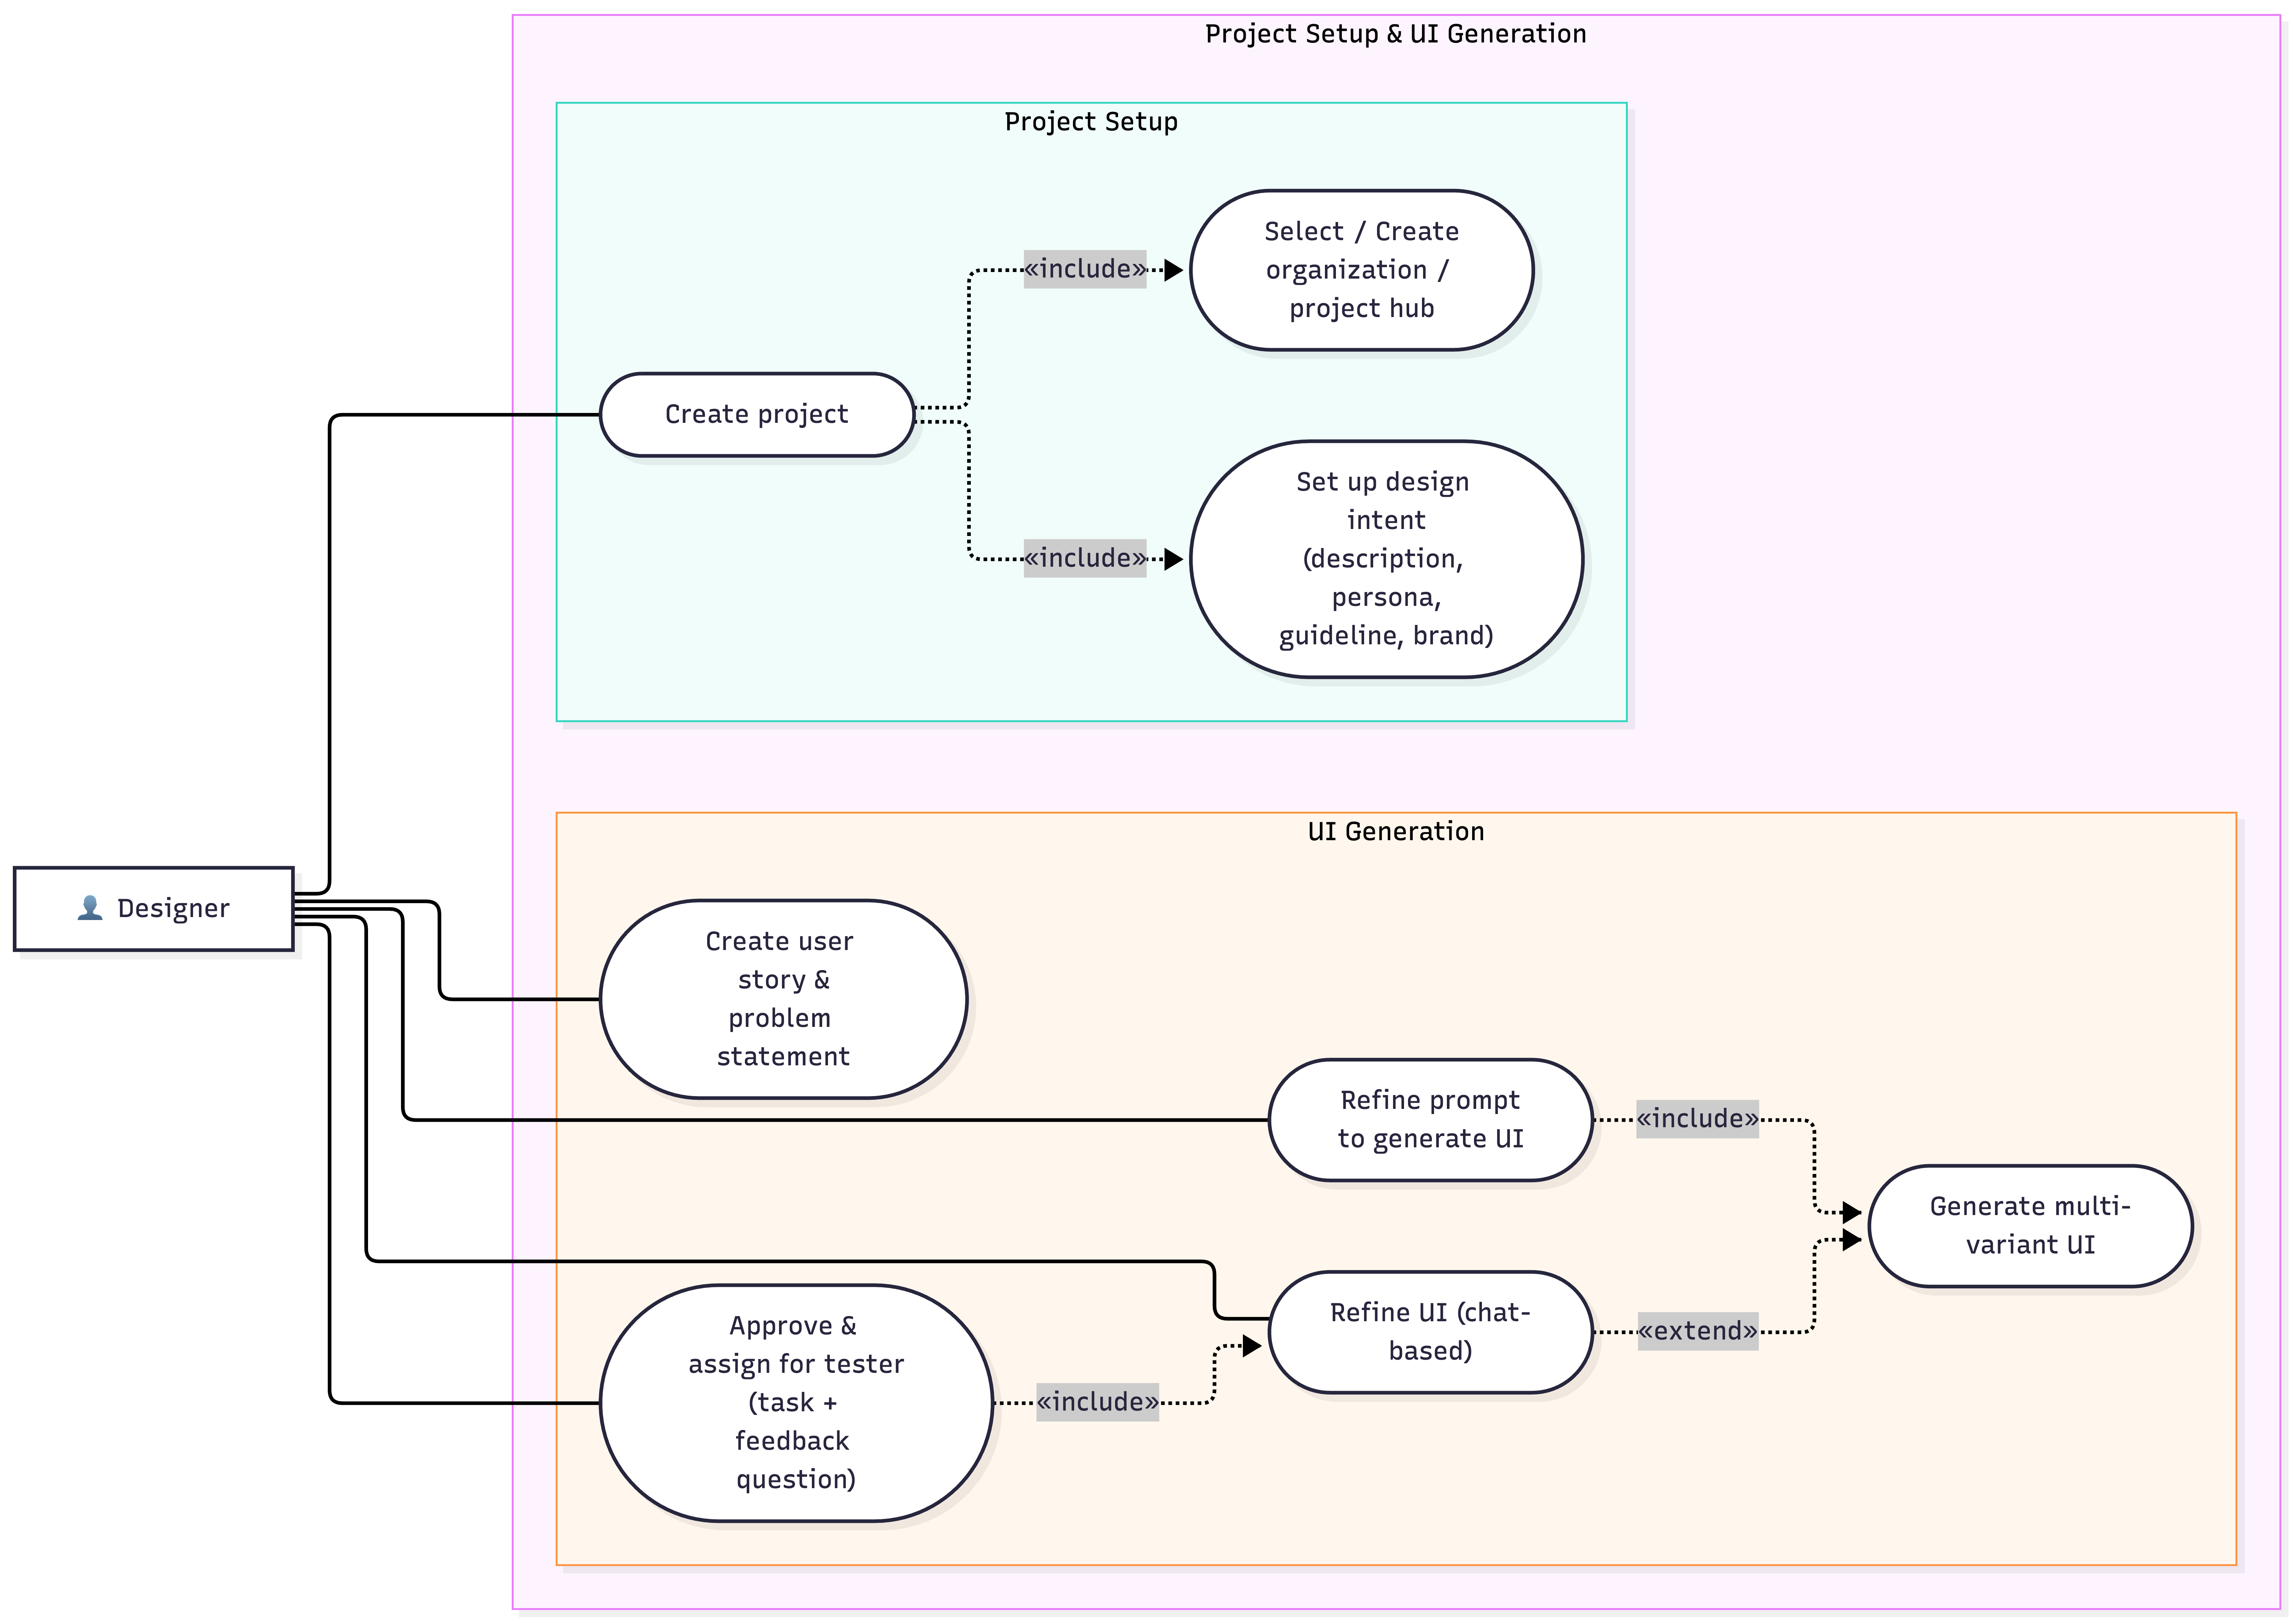
\includegraphics[
      width=0.6\textheight,
      height=\linewidth,
      keepaspectratio,
      origin=c
    ]{figures/ch3-methodology/UC-2.png}
    \caption{Use case diagram for Project setup and UI Generation}
    \label{fig:UC-2}
    \thaijustify{ภาพแสดง Use Case ของกระบวนการจัดเตรียมโครงการและสร้าง UI โดย Designer สามารถสร้างโครงการ กำหนด Design Intent สร้างและปรับแต่ง Prompt เพื่อสร้าง UI หลายรูปแบบ รวมถึงปรับแก้ UI และอนุมัติเพื่อส่งให้ผู้ทดสอบประเมิน}
  \end{figure}
  \subsection{Designer and Tester: Testing session and Feedback analysis}
  \begin{figure}[H]
    \centering
    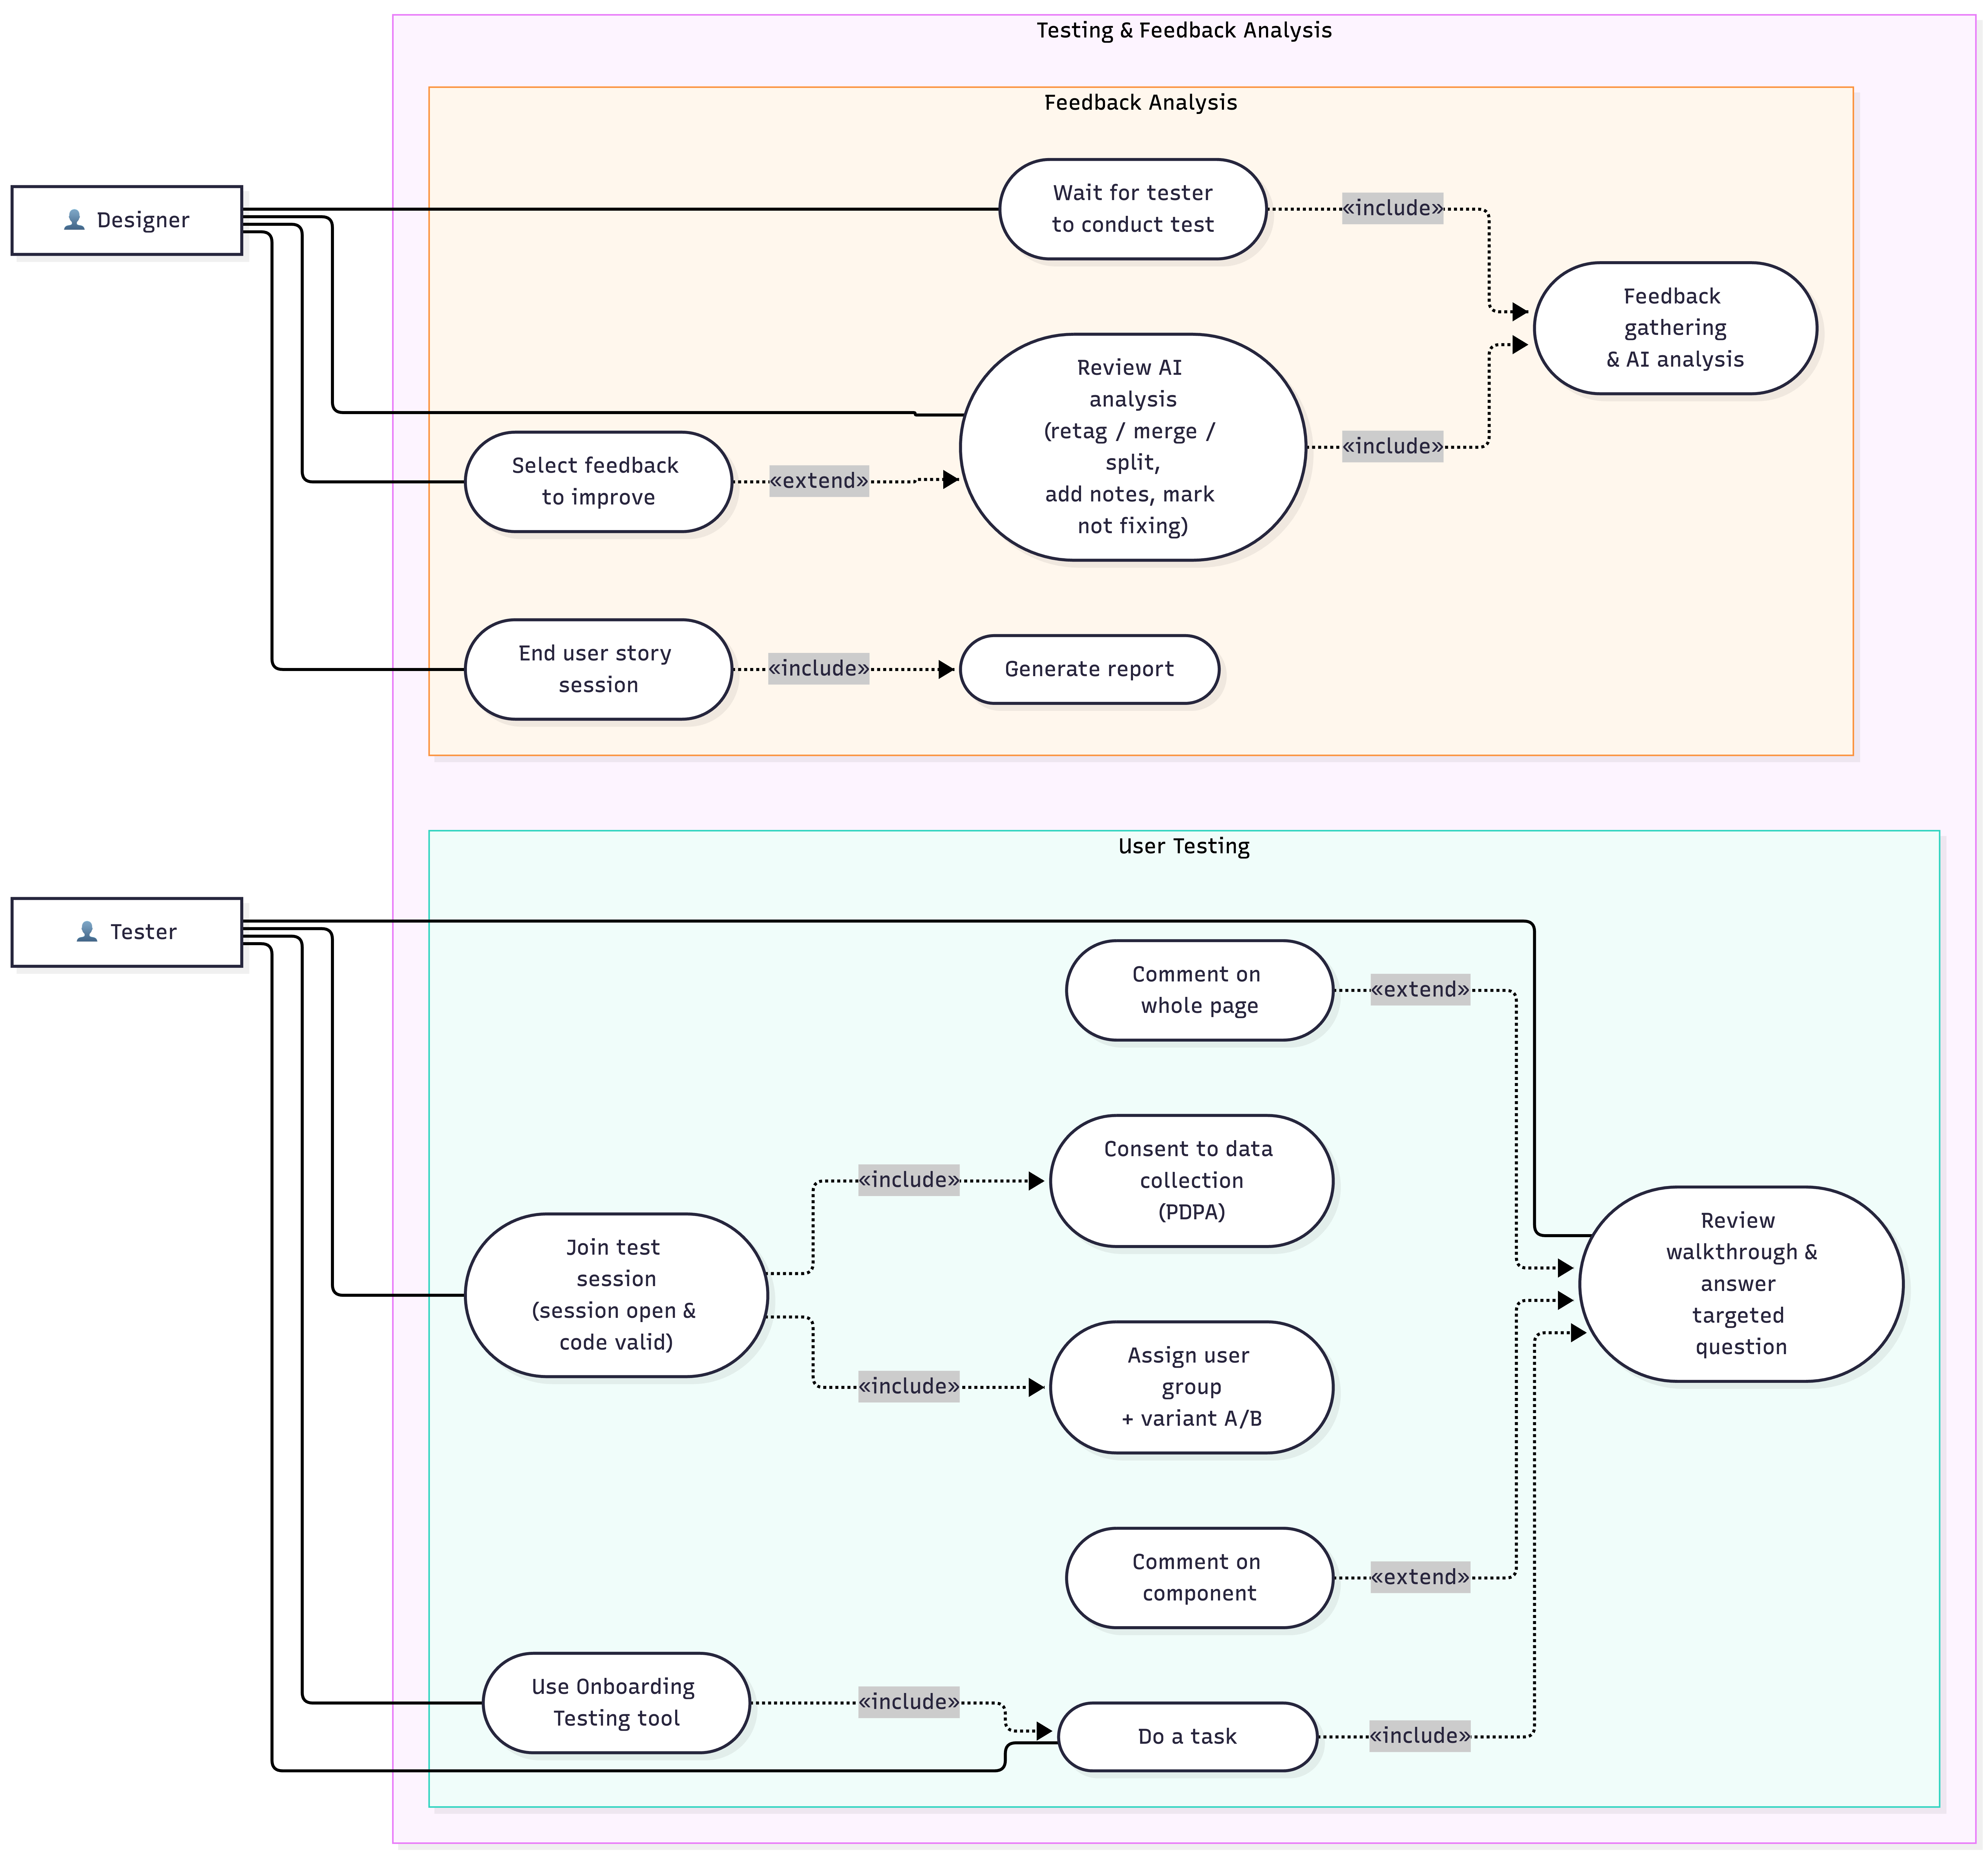
\includegraphics[
      width=0.6\textheight,
      height=\linewidth,
      keepaspectratio,
      origin=c
    ]{figures/ch3-methodology/UC-3.png}
    \caption{Use case diagram for Testing session and Feedback analysis}
    \label{fig:UC-3}
    \thaijustify{ภาพแสดง Use Case ของกระบวนการทดสอบและวิเคราะห์ Feedback โดย Tester เข้าร่วมการทดสอบ ทำภารกิจ และให้ความคิดเห็น ขณะที่ Designer รวบรวมและตรวจสอบผลการทดสอบ วิเคราะห์ Feedback ด้วย AI และเลือกประเด็นเพื่อนำไปปรับปรุงส่วนต่อประสานผู้ใช้}
  \end{figure}
  \subsection{Client, Developer, and Project Manager: Project view and Report}
  \begin{figure}[H]
    \centering
    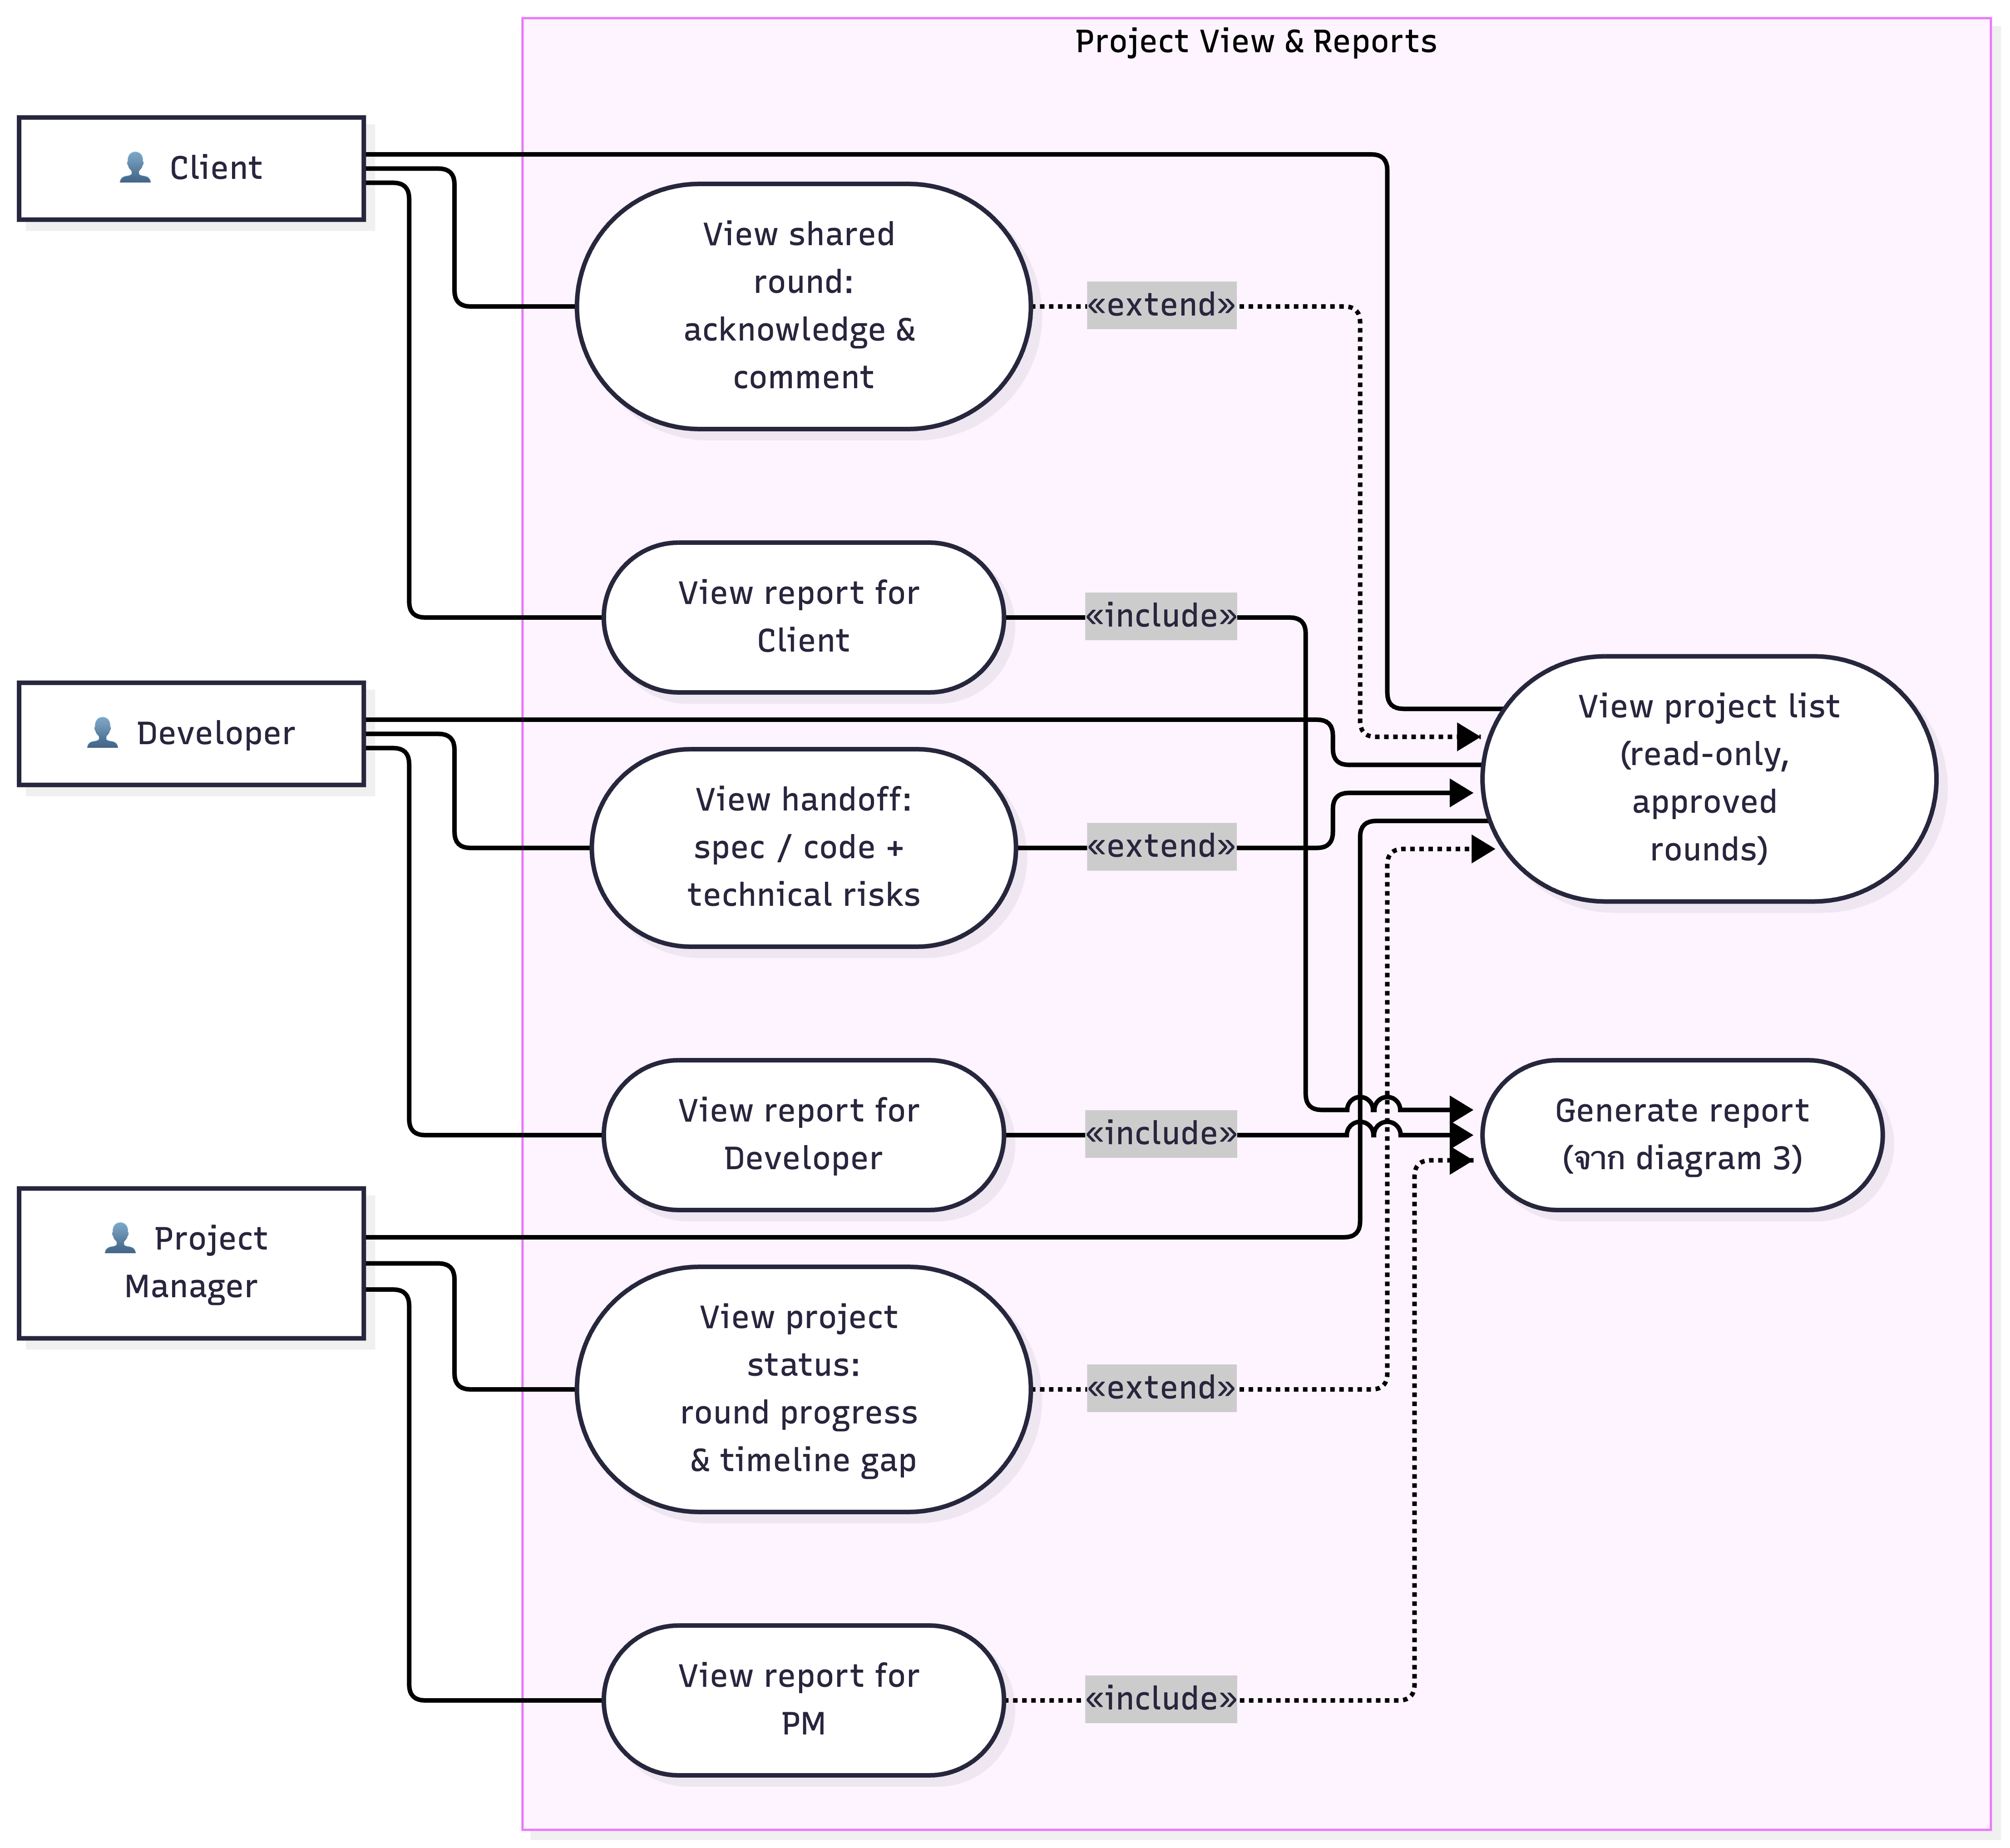
\includegraphics[
      width=0.6\textheight,
      height=\linewidth,
      keepaspectratio,
      origin=c
    ]{figures/ch3-methodology/UC-4.png}
    \caption{Use case diagram for Project view and Report}
    \label{fig:UC-4}
    \thaijustify{
      ภาพแสดง Use Case ของการดูโครงการและรายงาน โดย ผู้ใช้งาน, นักพัฒนา และ ผู้ดูแลโครงการ สามารถดูข้อมูลโครงการที่ได้รับอนุมัติและข้อมูลที่เกี่ยวข้องตามบทบาท รวมถึงดูรายงานที่สร้างจากผลการทดสอบและ Feedback
    }
  \end{figure}
\end{samepage}

\section{System Architecture \& Tech Stack}
\begin{figure}[H]
  \centering
  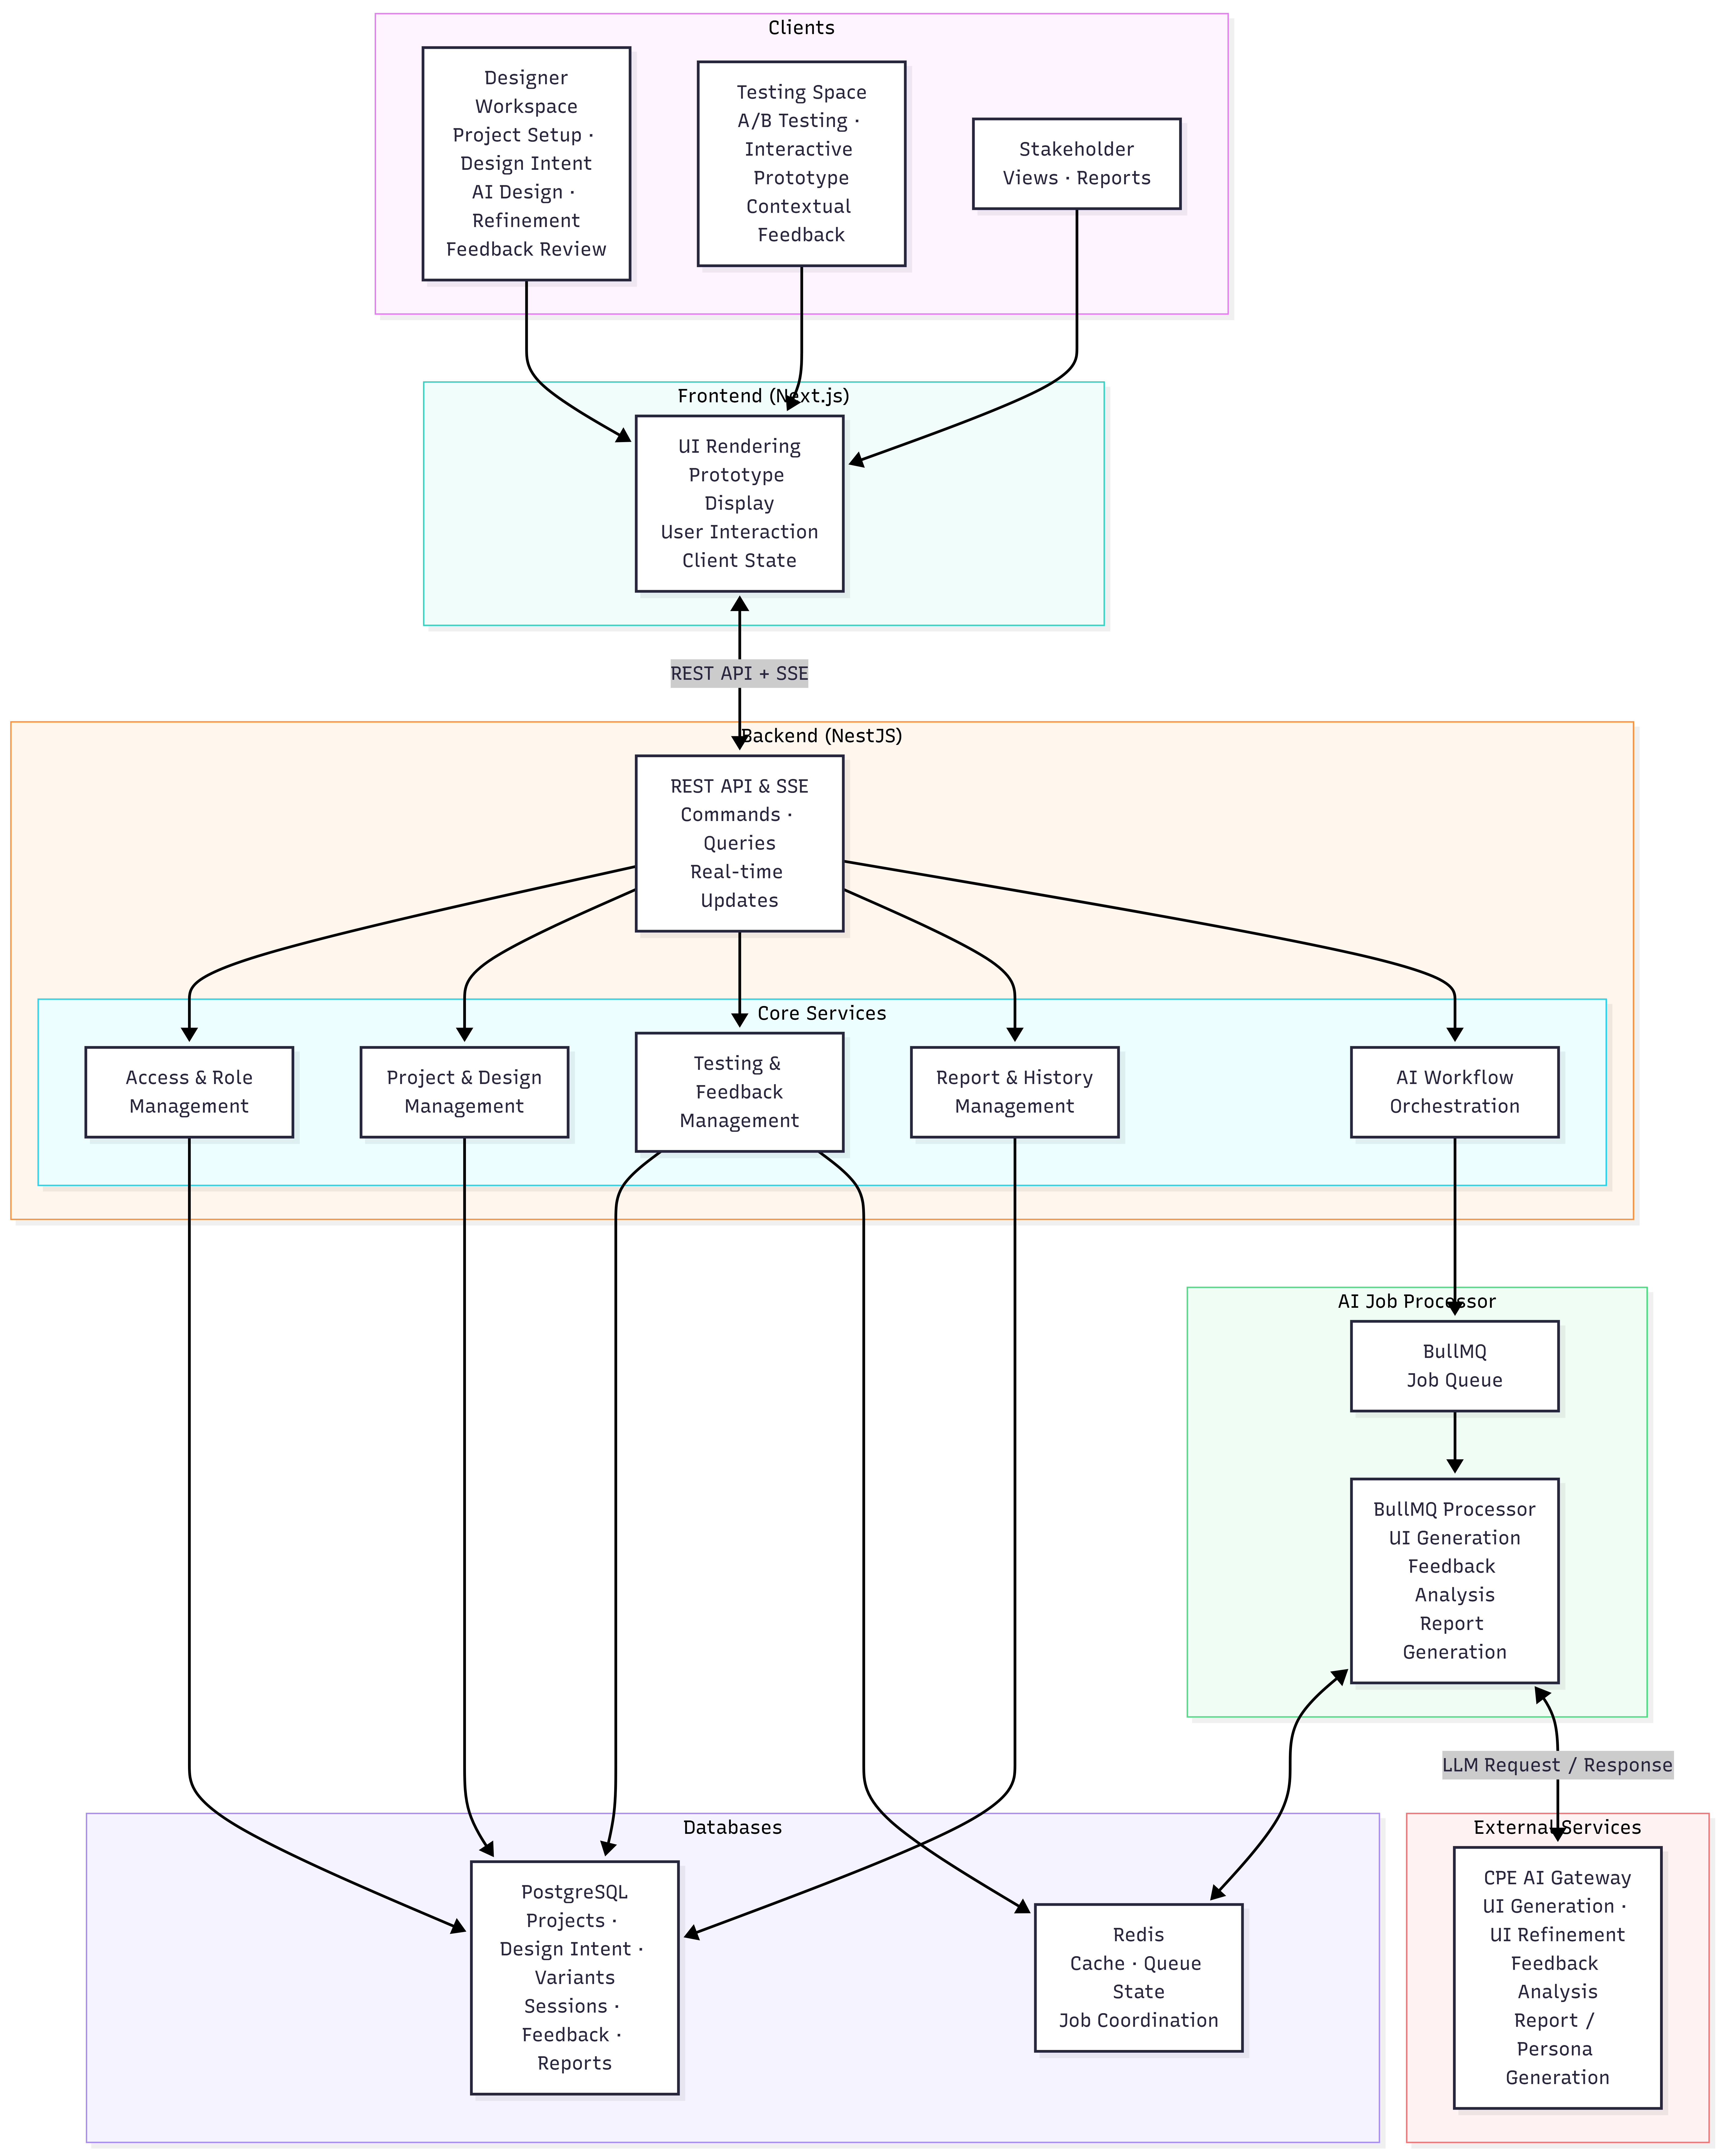
\includegraphics[
    width=0.8\linewidth,
    height=\textheight,
    keepaspectratio
  ]{figures/ch3-methodology/sys-arch3.png}
  \caption{System architecture}
  \label{fig:tech-stack-system-architecture}
  \thaijustify{ภาพแสดงสถาปัตยกรรมระบบโดยแบ่งออกเป็น Client, Frontend, Backend, AI Job Processor, Database และ External Services โดย Frontend พัฒนาด้วย Next.js และสื่อสารกับ Backend ผ่าน REST API และ SSE (Server-Sent Events) ซึ่งช่วยให้ Server สามารถส่งข้อมูลและการอัปเดตแบบ Real-time ไปยัง Client ได้โดยไม่ต้องส่ง Request ใหม่ ขณะที่ Backend ซึ่งพัฒนาด้วย NestJS ทำหน้าที่จัดการสิทธิ์ ข้อมูลโครงการ การทดสอบ Feedback รายงาน และกระบวนการ AI โดยงานที่ต้องใช้เวลาประมวลผลจะถูกส่งผ่าน BullMQ ไปยัง AI Job Processor และเชื่อมต่อกับ CPE AI Gateway สำหรับการประมวลผลด้วย AI}
\end{figure}

